\documentclass{beamer}

% Theme and color settings
\usetheme{Madrid}          % Clean, minimal theme
\usecolortheme{default}    % Simple color scheme

% Packages
\usepackage{graphicx}      % For images
\usepackage{amsmath}       % For math support
\usepackage{hyperref}      % For clickable links

% Title, author, date
\title{Pero si mi codigo corre en mi compu!}
\subtitle{Desarollo en Contenedores}
\author{Teresa Bracahamonte \& Nicolas Vega}
\date{\today}

\begin{document}

% Title slide
\begin{frame}
  \titlepage
\end{frame}

\begin{frame}{Acerca de}
  \begin{itemize}
    \item \textbf{Doctora Teresa Bracahamonte:} Experta en desarrollo de software y contenedores.
    \item \textbf{Nicolas Vega:} Ingeniero de software con experiencia en contenedores y DevOps.
  \end{itemize}
\end{frame}

% Table of contents
\begin{frame}{Agenda}
  \tableofcontents
\end{frame}

% Section 1
\section{Introduccion}
\subsection{Que son los entornos de desarrollo en contenedores?}
\begin{frame}{\subsecname}
  Los dev containers permiten tener un ambiente aislado con una serie de configuraciones 
  y features que ayudan a los desarolladores a correr sus aplicaciones mejorando la 
  integracion continua y testing.
  \begin{block}{En estos contenedores encontramos}
    \begin{itemize}
      \item Sistema operativo reducido (\textbf{imagen})
      \item Paquetes de ejecución y productividad (\textbf{features})
      \item Sistema de archivos locales del contenedor
      \item Nuestro código (\textbf{volumen} host:contenedor)
      \item Backend de nuestro IDE 
      \item Pueden correr en entornos locales o remotos
    \end{itemize}
  \end{block}
\end{frame}

\subsection{Detras de la caja negra}
\begin{frame}{\subsecname}
  \begin{figure}
    \centering
    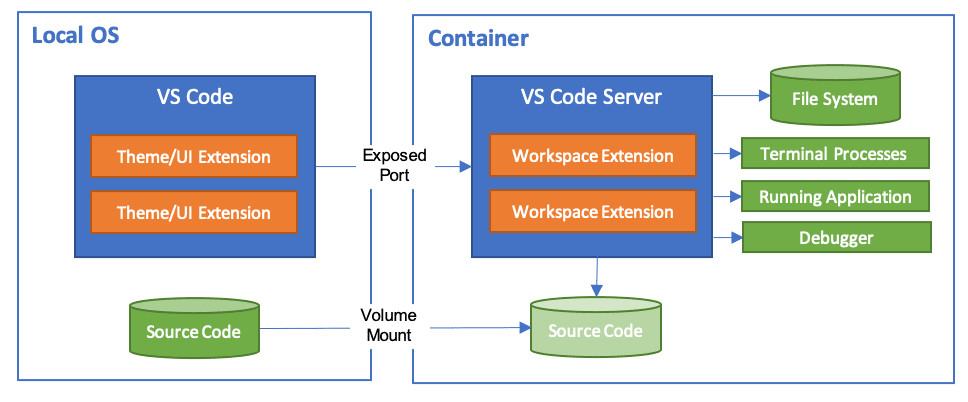
\includegraphics[width=\textwidth]{images/architecture-containers.png}
    \caption{Arquitectura de contenedores en entornos de desarrollo.}
  \end{figure}
\end{frame}

\subsection{Beneficios del desarrollo en contenedores}
\begin{frame}{\subsecname}
  \begin{itemize}
    \item \textbf{Aislamiento:} Cada proyecto puede tener su propio contenedor, lo cual previene conflictos entre diferentes versiones de dependencias en proyectos diferentes.
    \item \textbf{Portabilidad:} Funciona en cualquier máquina con Docker.
    \item \textbf{Consistencia:} Contenedores logran encapsular el entorno de desarrollo (librerías, dependencias, etc). Los desarrolladores logran un entorno de desarrollo consistente en todas sus máquinas locales.
    \item \textbf{Facilidad de uso:} Configuración rápida y sencilla.
  \end{itemize}
\end{frame}

\subsection{Desafios asociados al desarollo en contenedores}
\begin{frame}{\subsecname}
  \begin{itemize}
    \item \textbf{Curva de aprendizaje:} Requiere un conocimiento básico, comandos y herramientas relacionadas a contenedores. Esto podría volver lenta la adopción y aumentar la curva de aprendizaje de los desarrolladores.
    \item \textbf{Rendimiento:} El correr los contenedores en local requiere mayor utilización de memoria y CPU, sumado a que se pueden correr múltiples entornos de desarrollo a la vez.
    \item \textbf{Depuración:} Herramientas de depuración pueden ser limitadas.
    \item \textbf{Seguridad:} Los contenedores podrían tener vulnerabilidades o librerías desactualizadas.
  \end{itemize}
\end{frame}
\subsection{Ciclo de desarrollo ideal}
\begin{frame}{\subsecname}
  \begin{figure}
    \centering
    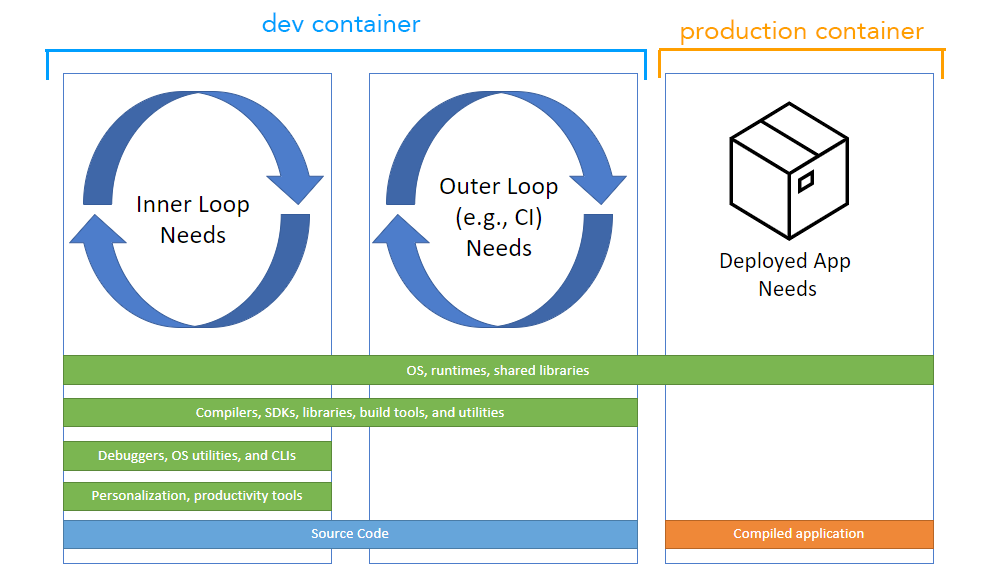
\includegraphics[width=\textwidth]{images/dev-container-stages.png}
    \caption{Dev,CI y Prod}
  \end{figure}
\end{frame}

\section{Setup Inicial}
\begin{frame}{Desarrollo local}
  \begin{block}{Docker}
    \begin{itemize}
      \item \textbf{Docker Desktop:} Herramienta de Docker para correr contenedores en local.
      \item \textbf{Docker CLI:} Interfaz de línea de comandos para interactuar con Docker.
    \end{itemize}
  \end{block}
  \begin{block}{Visual Studio Code}
    \begin{itemize}
      \item \textbf{Dev Containers:} Extensión de Visual Studio Code que permite crear y administrar contenedores de desarrollo.
      \item \textbf{Remote - SSH:} Extensión de Visual Studio Code que permite conectarse a máquinas remotas a través de SSH.
      \item \textbf{WSL:} Extensión de Visual Studio Code que permite trabajar con el Subsistema de Windows para Linux.
    \end{itemize}
  \end{block}
\end{frame}


\subsection{Python uv fastapi en entorno local}
\begin{frame}{\subsecname}
  \begin{columns}
    \begin{column}{0.7\textwidth}
      \begin{itemize}
        \small
        \item Get the project from github
        \item \href{https://github.com/copernicus231/devcontainer-boilerplate-python-uv-fastapi.git}{https://github.com/copernicus231/devcontainer-boilerplate-python-uv-fastapi.git}
        \item Ir a la paleta de comandos y buscar "Dev Containers: Reopen in Container"
        \item Seleccionar "Reopen in Container"
        \normalsize    \end{itemize}
      El contenedor se creara usando el archivo en \textbf{.devcontainer/devcontainer.json}
    \end{column}
    \begin{column}{0.3\textwidth}
      \begin{figure}
        \centering
        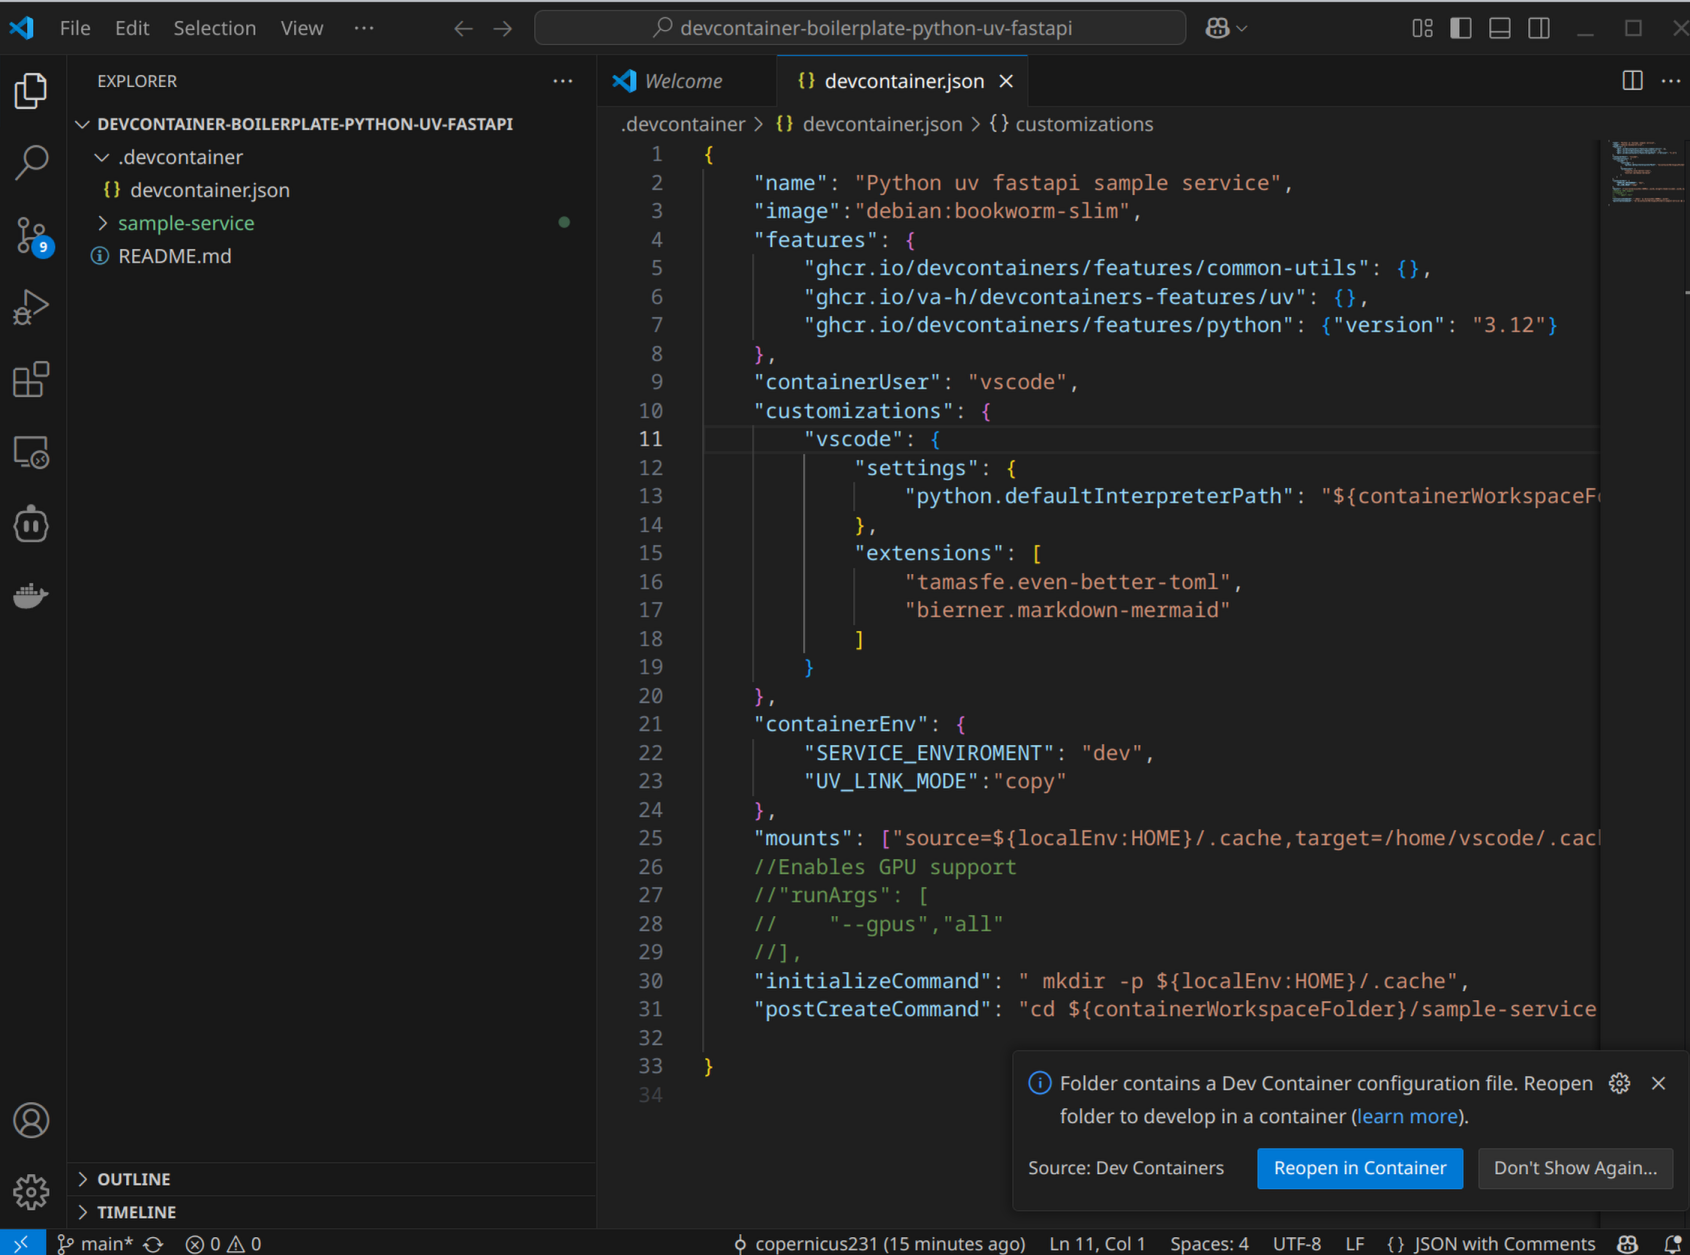
\includegraphics[width=\textwidth]{images/open-container.png}
        \caption{Configuración de FastAPI en contenedor.}
      \end{figure}
    \end{column}
  \end{columns}
\end{frame}

\begin{frame}{\subsecname}
  \begin{columns}
    \begin{column}{0.5\textwidth}
      \begin{itemize}
        \item \texttt{cd simple-service}
        \item \texttt{uv run fastapi dev src/simple\_service/base.py}
      \end{itemize}
        \end{column}
        \begin{column}{0.5\textwidth}
      \begin{figure}
        \centering
        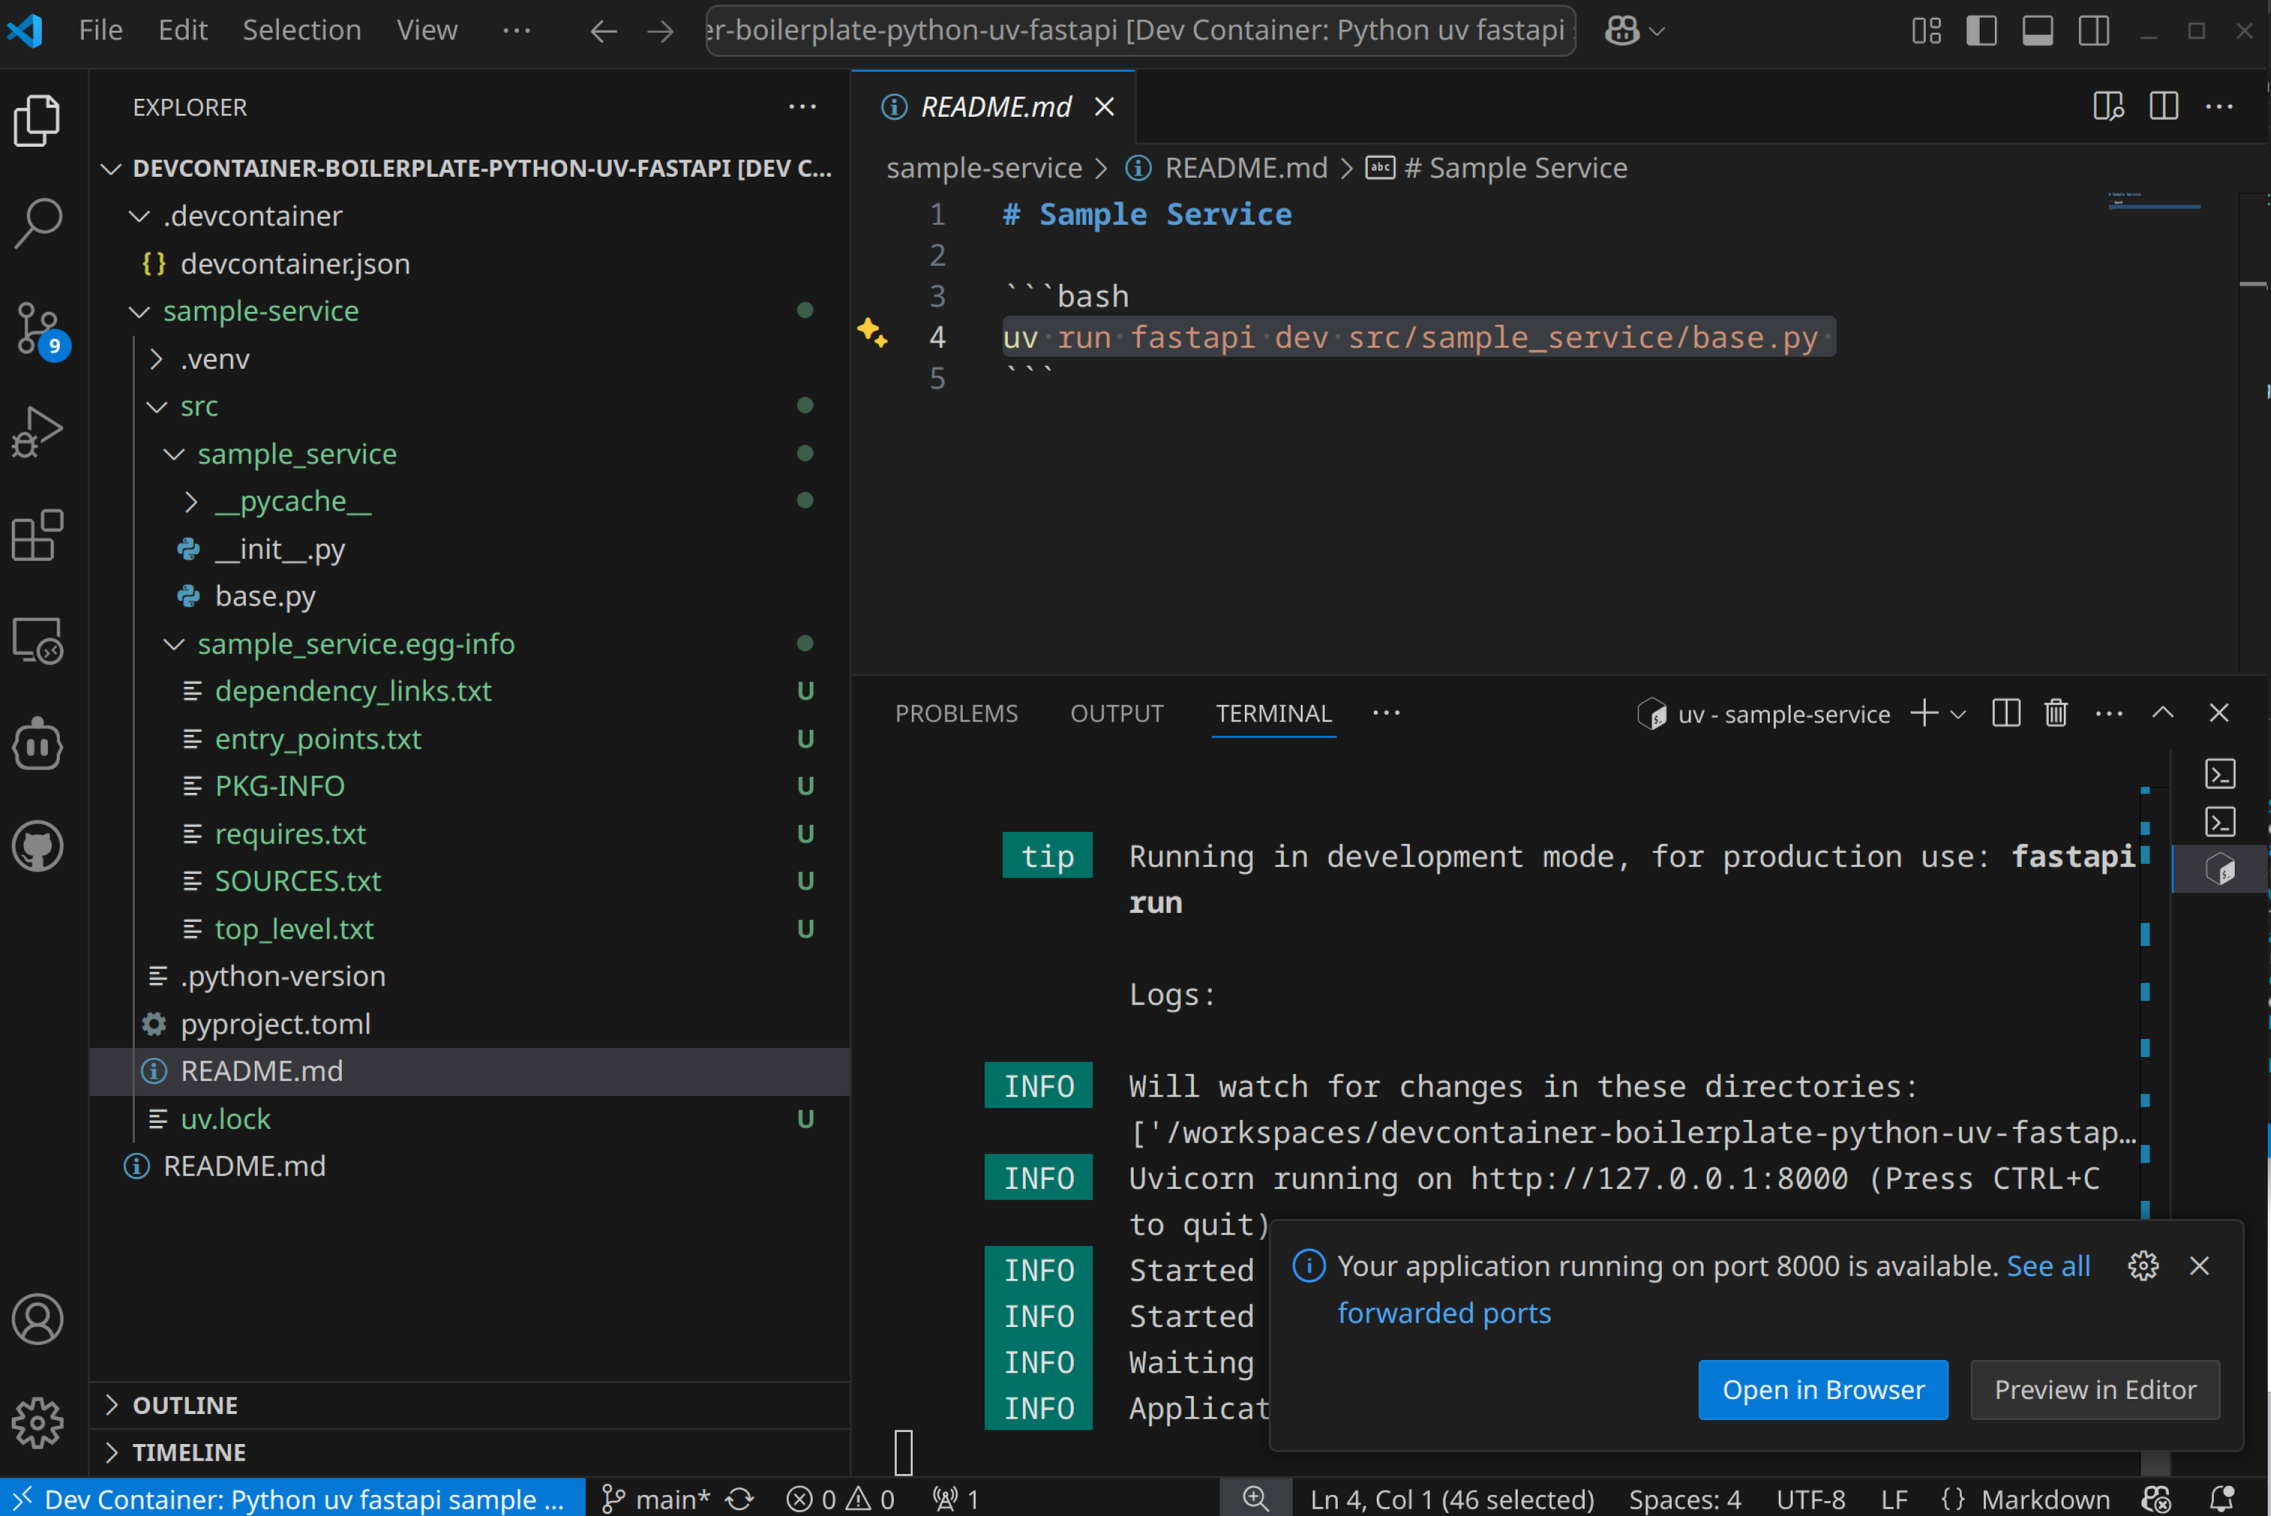
\includegraphics[width=\textwidth]{images/run-fastapi.png}
        \caption{Run fastapi endpoint}
      \end{figure}
        \end{column}
  \end{columns}
\end{frame}
\section{Archivos de configuracion}
\subsection{Devcontainer Spec}
\begin{frame}{\subsecname}

\end{frame}
\section{Conclusion}
\begin{frame}{Conclusion}
  \begin{itemize}
    \item \textbf{Key Takeaways:} Containers offer a powerful and efficient way to package and deploy applications.
    \item \textbf{Future Work:} Explore advanced containerization techniques like service meshes and serverless containers.
    \item \textbf{Thank You:} Thank you for your time and attention!
  \end{itemize}
\end{frame}

\end{document}
